% =============================================================================
% BrailleBridge — A Low-Cost Bilingual Braille Writing and Classroom
%                Examination System
%
% Author:  Samin Yeasar
% Contact: samin@mentormind.bd
% GitHub:  github.com/Solez-ai
% Web:     https://solez.html-5.me
% =============================================================================
\documentclass[11pt,a4paper,twoside]{article}

% Compile with XeLaTeX or LuaLaTeX for full Unicode (Bengali) support.
\usepackage{ifxetex}\usepackage{ifluatex}
\newif\ifxetexoru\ifxetex\xetexorutrue\else\ifluatex\xetexorutrue\fi\fi
\ifxetexoru
  \usepackage{fontspec}
  \setmainfont[Ligatures=TeX]{TeX Gyre Termes}
  \usepackage{newtxmath}
\else
  \PackageError{braillebridge}{Requires XeLaTeX or LuaLaTeX.\\MessageBreak
    Switch compiler: Overleaf Menu > Compiler > XeLaTeX}\stop
\fi
\usepackage[english]{babel}

\usepackage[top=2.5cm, bottom=2.5cm, left=2.8cm, right=2.8cm,
            headheight=14pt, footskip=1.2cm, includeheadfoot]{geometry}
\usepackage{microtype}
\usepackage{graphicx,xcolor,float,booktabs,array,longtable}
\usepackage{listings}
\usepackage[htt]{hyphenat}
\usepackage{tikz}
\usetikzlibrary{shapes.geometric,arrows,positioning,fit,backgrounds,calc}
\usepackage[european]{circuitikz}
\usepackage{hyperref}
\usepackage{tocloft,fancyhdr,enumitem,caption,verbatim,colortbl,textcomp}

\hypersetup{colorlinks=true,linkcolor=blue!60!black,citecolor=blue!60!black,
  urlcolor=blue!60!black,breaklinks=true,
  pdftitle={BrailleBridge --- Low-Cost Bilingual Braille System},
  pdfauthor={Samin Yeasar}}

\definecolor{deepnavy}{HTML}{0f111a}
\definecolor{richgold}{HTML}{C49A4A}
\definecolor{coolgrey}{HTML}{8A8A9A}
\definecolor{accentblue}{HTML}{3B82F6}
\definecolor{accentgreen}{HTML}{10B981}
\definecolor{codebg}{HTML}{F5F3F0}
\definecolor{lineshade}{HTML}{F0EFEA}

\lstset{language=C++,backgroundcolor=\color{codebg},
  basicstyle=\small\ttfamily,keywordstyle=\bfseries\color{deepnavy},
  stringstyle=\color{accentgreen},commentstyle=\itshape\color{coolgrey},
  numbers=left,numberstyle=\tiny\color{coolgrey},stepnumber=1,
  numbersep=8pt,frame=single,framerule=0.5pt,rulecolor=\color{lineshade},
  tabsize=2,breaklines=true,breakatwhitespace=true,
  showstringspaces=false,captionpos=t,xleftmargin=3.2em,
  aboveskip=1.2em,belowskip=0.8em,extendedchars=true}

\pagestyle{fancy}\fancyhf{}
\fancyhead[LE,RO]{\small\textsc{BrailleBridge}}
\fancyhead[RE,LO]{\small\thepage}
\renewcommand{\headrulewidth}{0.4pt}
\fancyfoot[C]{\small\textit{A Low-Cost Bilingual Braille Writing System}}
\setcounter{tocdepth}{3}\setcounter{secnumdepth}{3}

\newcommand{\projectname}{\textsc{BrailleBridge}}
\newcommand{\led}{\textsc{led}}
\newcommand{\bengali}[1]{#1}

\begin{document}

%% TITLE PAGE
\begin{titlepage}\centering\vspace*{1.8cm}
{\color{richgold}\rule{0.75\textwidth}{1.2pt}}\\[1.2em]\vspace{0.6cm}
{\Huge\bfseries\sffamily BrailleBridge}\\[0.3cm]
{\Large\itshape A Low-Cost Bilingual Braille Writing}\\
{\Large\itshape and Classroom Examination System}\\[1.2cm]
{\color{richgold}\rule{0.75\textwidth}{1.2pt}}\\[2cm]\vfill
\begin{minipage}{0.7\textwidth}\centering\large
\textbf{Author}\\[0.3em]{\Large\scshape Samin Yeasar}\\[0.8em]
\href{mailto:samin@mentormind.bd}{samin@mentormind.bd}\\[0.3em]
\href{https://github.com/Solez-ai}{github.com/Solez-ai}\\[0.3em]
\href{https://solez.html-5.me}{solez.html-5.me}\\[1.2em]
{\color{richgold}\rule{0.4\textwidth}{0.6pt}}\\[1em]
\small\textit{A project submitted for the}\\[0.2em]
\textit{Science \& Technology Innovation Competition}\\[0.2em]\vspace{1.2cm}\today
\end{minipage}\vfill\end{titlepage}

\clearpage\tableofcontents\clearpage

%% 1 — ABSTRACT
\section{Project Abstract}

\projectname{} is a low-cost, bilingual digital Braille writing system for
blind and visually impaired students to write independently during
classroom activities, tests, and examinations. Currently, many blind
students must dictate answers to a sighted writer, sacrificing privacy,
independence, and accuracy.

The device uses six mechanical keys (Braille dots 1--6) plus Space and
Shift keys. An ESP32 detects chorded key combinations, translates them
via embedded dictionaries into English, Bangla, numbers, punctuation, and
mathematical symbols, and sends output over Bluetooth (to the student's
device) and USB Serial (to the Teacher Software). The Teacher Software ---
built with HTML, CSS, and JavaScript using the Web Serial API --- displays
translated text in real time, allowing teachers who do not know Braille to
monitor, review, save, and assess answers.

\projectname{} benefits both student (independence, privacy, control over
speed) and teacher (readable digital output, saved records with timestamps,
multi-student monitoring, exam mode, and file export). The system costs
substantially less than conventional Braille equipment and uses locally
replaceable components.

\begin{figure}[H]\centering
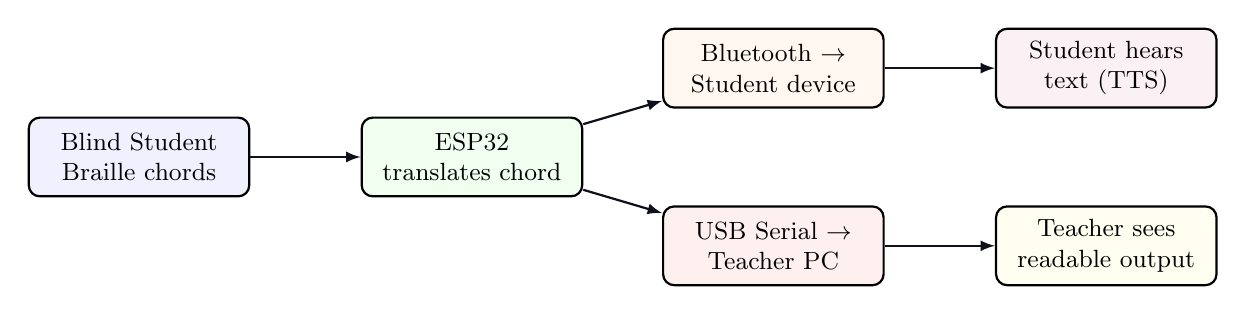
\begin{tikzpicture}[node distance=1.4cm,
  every node/.style={align=center,font=\small},
  box/.style={draw,rounded corners,fill=blue!6,minimum width=2.8cm,minimum height=1.0cm,thick},
  arrow/.style={-latex,thick,color=deepnavy}]
  \node[box,fill=blue!6] (student) {Blind Student\\Braille chords};
  \node[box,right=of student,fill=green!6] (esp32) {ESP32\\translates chord};
  \node[box,above right=0.1cm and 1.0cm of esp32,fill=orange!6] (bt) {Bluetooth $\rightarrow$\\Student device};
  \node[box,below right=0.1cm and 1.0cm of esp32,fill=red!6] (serial) {USB Serial $\rightarrow$\\Teacher PC};
  \node[box,right=1.4cm of bt,fill=purple!6] (studentView) {Student hears\\text (TTS)};
  \node[box,right=1.4cm of serial,fill=yellow!6] (teacherView) {Teacher sees\\readable output};
  \draw[arrow] (student)--(esp32); \draw[arrow] (esp32)--(bt);
  \draw[arrow] (esp32)--(serial); \draw[arrow] (bt)--(studentView);
  \draw[arrow] (serial)--(teacherView);
\end{tikzpicture}
\caption{High-level system architecture: a single chord produces dual output.}
\end{figure}

%% 2 — THE PROBLEM
\section{The Problem}

Blind students face barriers during written work. The common workaround ---
a sighted writer --- creates fundamental problems:

\begin{itemize}[nosep]
  \item \textbf{Loss of privacy:} Answers must be spoken aloud.
  \item \textbf{Loss of independence:} Someone else controls the final record.
  \item \textbf{Reduced speed control:} Student must wait for or repeat to the writer.
  \item \textbf{Transcription errors:} Technical terms, names, and Bangla
    phonetics are easily misheard.
  \item \textbf{Teacher accessibility gap:} Embossed Braille is unreadable to
    most sighted teachers.
  \item \textbf{Financial barriers:} Braille machines cost hundreds to thousands
    of dollars and are difficult to repair locally.
\end{itemize}

\projectname{} addresses this gap: the student writes independently via
familiar Braille chords, and the teacher receives ordinary digital text.

\begin{table}[H]\centering
\caption{Difficulties mapped to \projectname{} solutions.}\label{tab:problem-solution}
\begin{tabular}{p{0.4\textwidth} p{0.5\textwidth}}\toprule
\bfseries Difficulty & \bfseries \projectname{} Solution \\\midrule
Must dictate answers aloud & Silent Braille chord typing \\
No control over written record & Independent composition \\
Writer misunderstands terms & Direct chord-to-text translation \\
Teacher cannot read Braille & Digital text appears immediately \\
Expensive equipment & Low-cost ESP32 + switches \\\bottomrule
\end{tabular}\end{table}

%% 3 — INNOVATION
\section{Innovation and Novelty}

\projectname{} combines a physical Braille keyboard, bilingual translation,
Bluetooth output, and web-based teacher software --- all within one
affordable system. No existing product delivers this specific combination.

\subsection*{What makes \projectname{} different}
\begin{enumerate}[nosep]
  \item Six-dot physical Braille input with tactile mechanical switches.
  \item English and Bangla from the same hardware, with Shift-based modifiers
    for vowel signs, numbers, punctuation, and math.
  \item Bluetooth HID keyboard --- works with any device, no proprietary software.
  \item USB Serial output feeding a professional Teacher Software (HTML/CSS/JS).
  \item ESP32 architecture ($\sim$\$5) with Outemu switches ($\sim$\$0.38 each).
  \item Custom 3D-printed enclosure (Fusion~360 / FDM).
  \item Designed specifically for classrooms and examinations.
\end{enumerate}

\subsection*{Comparison with existing solutions}
\begin{table}[H]\centering
\caption{Comparison with alternatives.}\label{tab:comparison}
\begin{tabular}{p{2.8cm} p{3.8cm} p{4.8cm}}\toprule
\bfseries Solution & \bfseries Strength & \bfseries Limitation \\\midrule
Human writer & No equipment needed & Privacy loss, errors \\
Slate \& stylus & Affordable, tactile & Slow, teacher cannot read \\
Perkins Brailler & Familiar method & Expensive, heavy, embossed only \\
Voice typing & Fast in quiet & Fails in noisy classrooms \\
Commercial digital & Advanced accessibility & Very expensive, hard to repair \\
Ordinary keyboard & Cheap, ubiquitous & No six-dot chording \\
\rowcolor{lineshade}\projectname{} & Bilingual + teacher software & Prototype stage \\\bottomrule
\end{tabular}\end{table}

\subsection*{Novelty statement}
\projectname{} does not replace Braille --- it protects Braille as the
student's natural writing method while removing the barrier between
Braille input and teacher-readable output.

%% 4 — EXECUTIVE SUMMARY
\section{Project Summary --- What You Need to Know}

\projectname{} has two parts: a portable hardware device (six Braille keys,
Space, Shift, ESP32, LEDs, 3D-printed enclosure) and a web-based Teacher
Software (HTML/CSS/JS with Web Serial API).

\begin{table}[H]\centering
\caption{Specifications at a glance.}\label{tab:specs}
\begin{tabular}{l l}\toprule
\bfseries Parameter & \bfseries Value \\\midrule
Microcontroller & ESP32 Dev Module \\
Braille keys & 6 (Outemu Red mechanical switches) \\
Additional keys & Space, Shift \\
Chording window & 180\,ms \\
Output channels & Bluetooth HID + USB Serial \\
Languages & English, Bangla (Bharati Braille) \\
Shift functions & Caps, numbers, punctuation, math \\
LED indicators & Red (English), Green (Bangla) \\
Enclosure & Fusion 360 CAD, FDM 3D-printed \\
Teacher Software & HTML / CSS / JS (Web Serial API) \\
\bottomrule\end{tabular}\end{table}

\noindent\textbf{How it works (30 seconds):}
(1) Student presses Braille chords. (2) ESP32 collects keys within 180\,ms,
encodes as 6-bit value, looks up dictionary. (3) Character sent over
Bluetooth (student device) and USB Serial (Teacher Software).
(4) Teacher Software displays, timestamps, saves, and organises output.

\textbf{Cost:} Under \$15/device --- substantially less than mechanical
Braillers or commercial digital systems.

%% 5 — HARDWARE
\section{Hardware Architecture}

\subsection{ESP32 Microcontroller}
The ESP32 Dev Module is the central controller. It was selected because a
single chip provides everything the project needs: a dual-core Xtensa
LX6 processor running at 240\,MHz, 520\,KB SRAM, 4\,MB flash, and ---
critically --- integrated Bluetooth (BLE) and a USB-UART bridge for
programming and serial communication. The large GPIO count leaves ample
headroom: the eight switches, two LEDs, and future expansion (battery
monitoring, audio feedback) fit comfortably without multiplexing.

At roughly \$5 per module, the ESP32 costs a fraction of a dedicated
Braille display controller while offering the Arduino framework
ecosystem. The firmware uses the \texttt{BleKeyboard} library, which
registers the device as a standard Bluetooth HID keyboard, so no
proprietary receiver or driver is needed on the student's phone, tablet,
or computer.

\subsection{Mechanical Switches}
Eight Outemu Red switches form the input layer: six Braille dots, Space,
and Shift. Outemu Reds are MX-style linear mechanical switches rated for
approximately 50 million presses, giving a durable, consistent feel that
plain push-buttons cannot match. The linear action and audible click let
a blind student feel exactly when a key has registered, which is
essential for reliable chording.

Electrically each switch is trivial: one terminal connects to a GPIO and
the other connects to a shared ground bus. The firmware enables the
ESP32's internal pull-up resistors, so an unpressed key reads \texttt{HIGH}
and a pressed key connects the pin to ground and reads \texttt{LOW}. The
single common-ground bus keeps wiring short and the enclosure compact ---
only nine wires (eight switches + ground) reach the controller.

\subsection{GPIO Mapping}
The mapping below keeps the six Braille dots on consecutive, easily
routed pins, with Space and Shift grouped at the edge and the two LEDs on
the remaining outputs. Every switch shares a common ground, so only eight
signal wires plus one ground bus are required.

\begin{table}[H]\centering
\caption{GPIO mapping.}\label{tab:gpio}
\begin{tabular}{l c l}\toprule
\bfseries Function & \bfseries GPIO & \bfseries Notes \\\midrule
Dot 1 & 14 & Top-left \\
Dot 2 & 12 & Middle-left \\
Dot 3 & 13 & Bottom-left \\
Dot 4 & 27 & Top-right \\
Dot 5 & 26 & Middle-right \\
Dot 6 & 25 & Bottom-right \\
Space & 33 & Dedicated space key \\
Shift & 32 & Modifier \\
Red LED & 18 & English indicator \\
Green LED & 19 & Bangla indicator \\\bottomrule
\end{tabular}\end{table}

\subsection{LED Indicators}
Two status LEDs give instant, glanceable feedback without any audio. Each
LED is driven through a 220\,$\Omega$ current-limiting resistor from its
own GPIO (Red = GPIO~18, Green = GPIO~19). The state table is simple:

\begin{table}[H]\centering
\caption{LED state table.}\label{tab:led-states}
\begin{tabular}{l c c}\toprule
\textbf{State} & \textbf{Red LED} & \textbf{Green LED} \\\midrule
English mode & ON & OFF \\
Bangla mode & OFF & ON \\
Valid character (100\,ms flash) & ON & ON \\
Invalid chord (blinks three times) & blinks & blinks \\\bottomrule
\end{tabular}\end{table}

On power-up the device starts in English mode (red on). A successful
character flash is deliberately short (100\,ms) so the language colour is
restored almost immediately; an invalid chord blinks both LEDs three
times, mirroring the serial \texttt{Invalid} message sent to the Teacher
Software.

\subsection{3D-Printed Enclosure}
The enclosure is designed parametrically in Fusion~360 and printed on an
FDM printer in PLA (0.2\,mm layers, roughly 30\,g of filament per device).
The two-piece shell --- top and bottom --- secures together with M3
screws, and the switch plate uses MX-compatible cutouts so the eight
Outemu switches snap in without glue or solder. Design details include:

\begin{itemize}[nosep]
  \item Rounded outer corners for a comfortable desk profile.
  \item Raised tactile keycap markings so each dot key is identifiable by touch.
  \item Space and Shift keys positioned at the outer edges of the cell.
  \item LED openings with light-diffusing channels for the status lights.
  \item Internal cavity sized for the ESP32, wiring, and a future
    3.7\,V Li-ion cell with USB-C charging.
\end{itemize}

Because the design is a CAD model rather than a mould, any school or
hobbyist with an FDM printer can reproduce or repair it locally --- a
key part of the project's affordability and repairability story.

\subsection{Complete Circuit Diagram}
Figure~\ref{fig:circuit} shows the complete electrical circuit: the ESP32,
eight mechanical switches, two LEDs with current-limiting resistors, and the
common ground bus.

\begin{figure}[H]\centering
\resizebox{0.88\textwidth}{!}{%
\begin{circuitikz}[american]
  \node[font=\bfseries\Large] at (8,15) {BrailleBridge Hardware Wiring Diagram};
  \draw[fill=gray!15,rounded corners] (6,2) rectangle (10,13);
  \node[font=\bfseries] at (8,12.5){ESP32 DevKit};
  \node[left] at (6,11){GPIO14};
  \node[left] at (6,10){GPIO12};
  \node[left] at (6,9){GPIO13};
  \node[left] at (6,8){GPIO27};
  \node[left] at (6,7){GPIO26};
  \node[left] at (6,6){GPIO25};
  \node[left] at (6,5){GPIO33};
  \node[right] at (10,10){GPIO18};
  \node[right] at (10,9){GPIO19};
  \node[right] at (10,4){3.3V};
  \node[right] at (10,3){GND};
  \foreach \y/\name in {11/Dot 1,10/Dot 2,9/Dot 3,8/Dot 4,7/Dot 5,6/Dot 6,5/Space} {
    \draw (0,\y) node[left]{\name} to[push button,l=*] (2,\y);
    \draw (2,\y) -- (6,\y);
  }
  \draw[very thick] (2,3) -- (2,12);
  \node[left] at (2,12.4){GND Rail};
  \foreach \y in {11,10,9,8,7,6,5} { \draw (1,\y) -- (2,\y); }
  \draw (2,3) -- (6,3);
  \draw (10,10) -- (12,10) to[R,l=220$\Omega$] (14,10) to[led,l=Red] (14,8) -- (10,3);
  \node[right] at (14,10.6){English LED};
  \draw (10,9) -- (12,9) to[R,l=220$\Omega$] (16,9) to[led,l=Green] (16,7) -- (10,3);
  \node[right] at (16,9.6){Bangla LED};
  \draw[fill=blue!10] (7.2,13.2) rectangle (8.8,14);
  \node at (8,13.6){USB};
  \draw (12,4) to[battery1,l=3.7V Li-ion] (12,1);
  \draw (12,4)--(10,4);
  \draw (12,1)--(10,3);
  \node[right] at (12,2.5){Battery};
  \node[align=left,font=\small] at (8,-1) {
    Six Outemu Red Mechanical Switches\\
    Bluetooth HID Keyboard\\
    ESP32 DevKit\\
    English/Bangla Status LEDs\\
    Rechargeable Li-ion Battery\\
    Common Ground Wiring
  };
\end{circuitikz}}
\caption{Complete circuit diagram: ESP32, eight switches, two LEDs, common ground.}\label{fig:circuit}
\end{figure}

%% 6 — FIRMWARE
\section{Firmware Architecture}

Written in C++ (Arduino framework). Responsibilities:
(1) Configure pins \texttt{INPUT\_PULLUP}. (2) Read six Braille keys.
(3) Detect chord onset. (4) Collect keys within 180\,ms window.
(5) Encode as 6-bit value. (6) Select language dictionary.
(7) Look up chord. (8) Apply Shift modifiers. (9) Send over Bluetooth + Serial.
(10) Update LEDs. (11) Reject invalid chords.

\subsection{Chord Encoding}
Each Braille dot is assigned a unique bit position in an 8-bit integer:
dot~1 = bit~0, dot~2 = bit~1, dot~3 = bit~2, dot~4 = bit~3, dot~5 = bit~4,
dot~6 = bit~5. The firmware reads each GPIO pin and sets the corresponding
bit when the pin is LOW (pressed). The resulting 6-bit value uniquely
identifies the chord. For example, pressing dots~1 and~4 simultaneously
produces the value \texttt{0b001001} (bits~0 and~3 set).

\begin{lstlisting}[caption=Reading GPIOs into a chord value.]
uint8_t readChord() {
  uint8_t chord = 0;
  if (digitalRead(PIN_DOT1) == LOW) chord |= (1 << 0);
  if (digitalRead(PIN_DOT2) == LOW) chord |= (1 << 1);
  if (digitalRead(PIN_DOT3) == LOW) chord |= (1 << 2);
  if (digitalRead(PIN_DOT4) == LOW) chord |= (1 << 3);
  if (digitalRead(PIN_DOT5) == LOW) chord |= (1 << 4);
  if (digitalRead(PIN_DOT6) == LOW) chord |= (1 << 5);
  return chord;
}
\end{lstlisting}

\subsection{Chording Window}
Because human fingers rarely press all keys within the same microsecond,
the firmware uses a timed collection window. When the first key is
detected, a timer starts. All additional keys pressed within the next
180\,ms are OR-ed into the same chord value. When the window expires,
the complete chord is processed and the system resets for the next input.
This prevents a single intentional chord from being misinterpreted as
multiple sequential keystrokes.

\begin{lstlisting}[caption=Chord detection with 180\,ms window.]
void loop() {
  uint8_t current = readChord();
  if (current > 0 && !chordingActive) {
    chordingActive = true; chordStartTime = millis(); chord = current;
  }
  if (chordingActive) {
    chord |= readChord();
    if (millis() - chordStartTime >= 180) {
      handleChord(chord & 0x3F); chordingActive = false;
    }
  }
}
\end{lstlisting}

\subsection{Dictionary Data Structure}
Rather than using large switch-case blocks, the firmware stores translations
in a structured array of \texttt{BrailleEntry} records. Each entry contains
the 6-bit chord value and the corresponding output string for English and
Bangla. A linear search function iterates through the array and returns the
correct language output or \texttt{nullptr} if no match is found. This design
makes it straightforward to add new characters or entire new languages ---
simply append entries to the array.

\begin{lstlisting}[caption=Braille dictionary entry and lookup.]
struct BrailleEntry { uint8_t chord; const char* english; const char* bangla; };

const char* lookup(const BrailleEntry* dict, int size,
                   uint8_t chord, bool isBangla) {
  for (int i = 0; i < size; i++)
    if (dict[i].chord == chord)
      return isBangla ? dict[i].bangla : dict[i].english;
  return nullptr;
}
\end{lstlisting}

\subsection{Language Switching}
\projectname{} needs no physical language switch. The active language is
toggled with a deliberate chord: dots 4, 5, and 6 pressed together and
held for 500\,ms. This combination was chosen because no standard
letter, number, or symbol chord uses exactly dots 4+5+6, so accidental
switching is practically impossible. A short press of the same three
dots is simply ignored --- only a sustained hold triggers the toggle.

The 500\,ms hold is measured with the same millisecond timer used by the
chording window. When the accumulated chord equals \texttt{0b111000}
(bits 3, 4, and 5) and the hold exceeds 500\,ms, the firmware flips the
\texttt{isBangla} flag, announces the new state on the serial line
(\texttt{LANG:en} or \texttt{LANG:bn}), and waits for the keys to be
released before accepting the next chord. The Teacher Software watches
for these status messages and updates its per-student language
indicator automatically.

The two status LEDs confirm the active language at a glance:

\begin{table}[H]\centering
\caption{Language state and LED indication.}\label{tab:lang-led}
\begin{tabular}{l c c}\toprule
\textbf{Language} & \textbf{Red LED} & \textbf{Green LED} \\\midrule
English & ON & OFF \\
Bangla & OFF & ON \\
Valid character (100\,ms flash) & ON & ON \\\bottomrule
\end{tabular}\end{table}

\begin{lstlisting}[caption=Language toggle detection in the main loop.]
if (currentChord == 0b111000 && elapsed >= 500) {
  isBangla = !isBangla;
  Serial.println(isBangla ? "LANG:bn" : "LANG:en");
  chordActive = false; currentChord = 0;
  while (digitalRead(DOT_4) == LOW || digitalRead(DOT_5) == LOW
      || digitalRead(DOT_6) == LOW) { delay(10); }
  return;
}
\end{lstlisting}

\subsection{Shift Behaviour}
The physical Shift key (GPIO~32) behaves like the modifier on a
conventional keyboard: the student holds it down while pressing a
Braille chord, and the firmware interprets that chord through a second
set of dictionaries. The priority is fixed so the result is always
predictable --- numbers first, then math and punctuation symbols, then
uppercase letters in English mode or vowel signs in Bangla mode.

\begin{table}[H]\centering
\caption{Shift modifier outputs.}\label{tab:shift-outputs}
\begin{tabular}{l l}\toprule
\textbf{Shift + chord} & \textbf{Output} \\\midrule
Shift + A--J & Numbers 1--0 \\
Shift + math chord & $+$, $-$, $\times$, $\div$, $=$ \\
Shift + punctuation chord & , ; : . \\
Shift + letter (English) & Uppercase letter \\
Shift + vowel (Bangla) & Vowel sign (\bengali{কার}) \\\bottomrule
\end{tabular}\end{table}

In English mode, Shift turns a base letter into its uppercase form, so
Shift + a produces \texttt{A}. In Bangla mode the same key
generates the dependent vowel signs (\bengali{কার}): for example,
Shift + \bengali{উ} (dots 1,3,6) yields \bengali{ূ}, allowing conjuncts
and vowel signs to be typed without leaving Bangla mode. All of this is
handled inside a single dispatch routine:

\begin{lstlisting}[caption=Shifted-chord dispatch.]
if (shiftActive) {
  for (int i = 0; i < 10; i++)                  // Shift + A--J = 1--0
    if (chord == numberChords[i]) { sendChar(numberMap[i]); return; }
  for (unsigned i = 0; i < sizeof(shiftSymbols)/sizeof(shiftSymbols[0]); i++)
    if (chord == shiftSymbols[i].chord) { sendChar(shiftSymbols[i].symbol); return; }
  if (!isBangla) {                              // English uppercase
    const char* ch = lookupChord(chord, false);
    if (ch && ch[0] >= 'a' && ch[0] <= 'z') {
      char upper[2] = { (char)(ch[0] - 32), '\0' };
      sendChar(upper);
    }
    return;
  }
  for (unsigned i = 0; i < sizeof(banglaShiftMap)/sizeof(banglaShiftMap[0]); i++)
    if (banglaShiftMap[i].chord == chord && banglaShiftMap[i].kar)
      { sendChar(banglaShiftMap[i].kar); return; }
  const char* ch = lookupChord(chord, true);
  if (ch) sendChar(ch);
}
\end{lstlisting}

\subsection{Translation Pipeline Flowchart}
Figure~\ref{fig:pipeline} summarises the complete chord-to-character
pipeline. Every chord --- from finger press to character output ---
passes through the same ten stages:

\begin{enumerate}[nosep]
  \item \textbf{Chord pressed} --- one or more Braille dot keys go LOW.
  \item \textbf{GPIO read} --- the six dot pins are sampled.
  \item \textbf{180\,ms window} --- additional keys pressed within the
    window are merged into the same chord.
  \item \textbf{6-bit mask} --- the accumulated keys are encoded as one
    six-bit value (dot 1 = bit 0 \ldots\ dot 6 = bit 5).
  \item \textbf{Shift pressed?} --- if Shift is held, the shifted
    dictionaries are searched; otherwise the main dictionaries are used.
  \item \textbf{Which language?} --- English or Bangla dictionary is
    selected.
  \item \textbf{Found chord?} --- a match produces the output character;
    a miss produces a rejection.
  \item \textbf{Output char} --- the character is sent over Bluetooth and
    USB Serial.
  \item \textbf{Flash} --- both LEDs flash for 100\,ms to confirm a valid
    character.
  \item \textbf{Wait} --- the system resets and waits for the next chord.
\end{enumerate}

Unknown chords are rejected quietly: both LEDs blink three times and the
serial line prints \texttt{Invalid}, so the Teacher Software can flag the
input without interrupting the student's flow.

\paragraph{Worked example: typing the letter C.}
Tracing one chord through the pipeline makes the stages concrete.
Suppose the student presses dots 1 and 4 together in English mode:

\begin{enumerate}[nosep]
  \item \textbf{Chord pressed} --- dot 1 and dot 4 go LOW simultaneously.
  \item \textbf{GPIO read} --- both pins sample LOW.
  \item \textbf{180\,ms window} --- no further keys arrive; the window
    closes and the chord is frozen.
  \item \textbf{6-bit mask} --- bit 0 (dot 1) and bit 3 (dot 4) set:
    \texttt{0b001001}.
  \item \textbf{Shift pressed?} --- no, Shift is released.
  \item \textbf{Which language?} --- English.
  \item \textbf{Found chord?} --- \texttt{lookupChord(0b001001, false)}
    returns \texttt{"c"}.
  \item \textbf{Output char} --- \texttt{sendChar("c")} writes to both
    Bluetooth and USB Serial.
  \item \textbf{Flash} --- both LEDs flash for 100\,ms.
  \item \textbf{Wait} --- the system resets for the next chord.
\end{enumerate}

The same chord in Bangla mode returns \texttt{চ} instead --- only the
dictionary changes, never the pipeline.

\paragraph{Mapping stages to firmware.}
Each pipeline stage corresponds to a specific part of the firmware:

\begin{table}[H]\centering
\caption{Pipeline stages and their firmware counterparts.}\label{tab:pipeline-map}
\begin{tabular}{p{3.2cm} p{8cm}}\toprule
\textbf{Pipeline stage} & \textbf{Firmware counterpart} \\\midrule
GPIO read & Six \texttt{digitalRead()} calls on the dot pins \\
180\,ms window & \texttt{millis()} timer in \texttt{loop()} \\
6-bit mask & Bitwise OR of \texttt{(1 << n)} per pressed dot \\
Shift pressed? & \texttt{shiftActive} flag from the Shift pin \\
Which language? & \texttt{isBangla} boolean flag \\
Found chord? & \texttt{lookupChord()} linear search of \texttt{brailleDict} \\
Output char & \texttt{sendChar()} over BLE + Serial \\
Flash / Wait & LED helpers and loop reset \\\bottomrule
\end{tabular}\end{table}

On a 240\,MHz dual-core ESP32 each lookup is a few microseconds, so the
entire pipeline completes well within the 180\,ms window --- typing feel
is immediate even with the largest dictionary.

\begin{figure}[H]\centering\scalebox{0.72}{\begin{tikzpicture}[node distance=1.0cm and 1.2cm,
  every node/.style={align=center,font=\small},
  startstop/.style={draw,rounded corners=4pt,minimum width=2.2cm,minimum height=0.6cm,thick,fill=deepnavy!6},
  process/.style={draw,rectangle,minimum width=2.2cm,minimum height=0.6cm,thick,fill=blue!6},
  decision/.style={draw,diamond,minimum width=2.0cm,minimum height=0.6cm,thick,fill=yellow!10,aspect=1.4},
  arrow/.style={-latex,thick,color=deepnavy!80},
  reject/.style={draw,rectangle,minimum width=2.0cm,minimum height=0.5cm,thick,fill=red!8,rounded corners}]
  \node[startstop] (start) {Chord\npressed};
  \node[process,below=of start] (gpio) {GPIO read};
  \draw[arrow] (start)--(gpio);
  \node[process,below=of gpio] (window) {180\,ms\nwindow};
  \draw[arrow] (gpio)--(window);
  \node[process,below=of window] (encode) {6-bit\nmask};
  \draw[arrow] (window)--(encode);
  \node[decision,below=of encode] (shiftQ) {Shift\npressed?};
  \draw[arrow] (encode)--(shiftQ);
  \node[process,right=2.0cm of shiftQ] (shiftDicts) {Shift\ndicts};
  \draw[arrow] (shiftQ.east)--node[above]{\tiny Yes}(shiftDicts.west);
  \node[decision,below=0.8cm of shiftQ] (langQ) {Which\nlang?};
  \draw[arrow] (shiftQ.south)--node[right]{\tiny No}(langQ.north);
  \node[decision,right=2.0cm of langQ] (shiftFoundQ) {Found\nchord?};
  \draw[arrow] (shiftDicts)--(shiftFoundQ);
  \node[process,below=of langQ] (mainLookup) {Main\ndict};
  \draw[arrow] (langQ.south)--(mainLookup.north);
  \node[process,below=0.8cm of shiftFoundQ] (sendShift) {Output\nchar};
  \draw[arrow] (shiftFoundQ.south)--node[right]{\tiny Yes}(sendShift.north);
  \node[decision,below=of mainLookup] (foundQ) {Found\nchord?};
  \draw[arrow] (mainLookup)--(foundQ);
  \node[process,below=of foundQ] (sendMain) {Output\nchar};
  \draw[arrow] (foundQ.south)--node[right]{\tiny Yes}(sendMain.north);
  \node[reject,right=2.0cm of foundQ] (invalid) {Invalid\nchord};
  \draw[arrow] (foundQ.east)--node[above]{\tiny No}(invalid.west);
  \draw[arrow,dashed] (shiftFoundQ.east)--++(0.6,0)|-(invalid.east);
  \node[below=of invalid] (endInv) {Wait};
  \draw[arrow] (invalid)--(endInv);
  \node[process,below=of sendMain] (flashV) {Flash};
  \draw[arrow] (sendMain)--(flashV);
  \node[process,below=of sendShift] (flashS) {Flash};
  \draw[arrow] (sendShift)--(flashS);
  \node[startstop,below=of flashV] (endM) {Wait};
  \node[startstop,below=of flashS] (endS) {Wait};
  \draw[arrow] (flashV)--(endM); \draw[arrow] (flashS)--(endS);
\end{tikzpicture}}
\caption{Chord-to-character translation pipeline.}\label{fig:pipeline}\end{figure}

%% 7 — DUAL COMMUNICATION
\section{Dual Communication Path}

Every translated character is sent through two independent channels:\begin{figure}[H]\centering
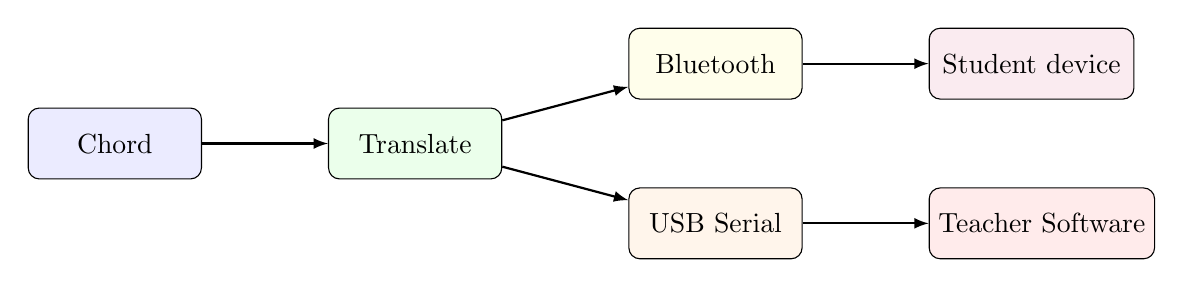
\begin{tikzpicture}[node distance=1.4cm, auto]
  \node[draw,rounded corners,fill=blue!8,minimum width=2.2cm,minimum height=0.9cm] (chord) {Chord};
  \node[draw,rounded corners,fill=green!8,minimum width=2.2cm,minimum height=0.9cm,right=1.6cm of chord] (translate) {Translate};
  \node[draw,rounded corners,fill=yellow!8,minimum width=2.2cm,minimum height=0.9cm,above right=0.1cm and 1.6cm of translate] (bt) {Bluetooth};
  \node[draw,rounded corners,fill=orange!8,minimum width=2.2cm,minimum height=0.9cm,below right=0.1cm and 1.6cm of translate] (serial) {USB Serial};
  \node[draw,rounded corners,fill=purple!8,minimum width=2.6cm,minimum height=0.9cm,right=1.6cm of bt] (student) {Student device};
  \node[draw,rounded corners,fill=red!8,minimum width=2.6cm,minimum height=0.9cm,right=1.6cm of serial] (teacher) {Teacher Software};
  \draw[-latex,thick] (chord)--(translate);
  \draw[-latex,thick] (translate)--(bt); \draw[-latex,thick] (translate)--(serial);
  \draw[-latex,thick] (bt)--(student); \draw[-latex,thick] (serial)--(teacher);
\end{tikzpicture}
\caption{Dual communication path.}\label{fig:dual-path}\end{figure}

Figure~\ref{fig:dual-path} illustrates this architecture.

\subsection{Bluetooth Output}
ESP32 as Bluetooth HID keyboard. No proprietary receiver needed. On the
student's paired phone, tablet, or computer, the typed text is spoken
aloud by the device's built-in screen reader (text-to-speech), so the
student receives immediate audible confirmation without needing to see
a screen.

\subsection{USB Serial Output}
The same character that leaves over Bluetooth is also written to the USB
serial line at 115200~baud, where the Teacher Software reads it through
the browser's Web Serial API. The protocol is deliberately minimal ---
all translation happens on the ESP32, so the wire carries only results:

\begin{table}[H]\centering
\caption{Serial protocol.}\label{tab:serial-protocol}
\begin{tabular}{l l}\toprule
\textbf{Message} & \textbf{Meaning} \\\midrule
\texttt{LANG:en} & Language switched to English \\
\texttt{LANG:bn} & Language switched to Bangla \\
\texttt{Invalid} & Unrecognised chord rejected \\
\texttt{<char>} & A translated character \\\bottomrule
\end{tabular}\end{table}

The \texttt{LANG:} messages let the Teacher Software update its per-student
language indicator without any student-side configuration, and every
character arrives already translated --- the teacher never has to decode
Braille themselves.

%% 8 — ENGLISH BRAILLE
\section{English Braille Dictionary}

Follows standard English Braille (Grade 1) for A--Z.

\subsection{Braille Cell Structure}
Figure~\ref{fig:braille-cell} shows the standard six-dot cell.

\begin{figure}[H]\centering
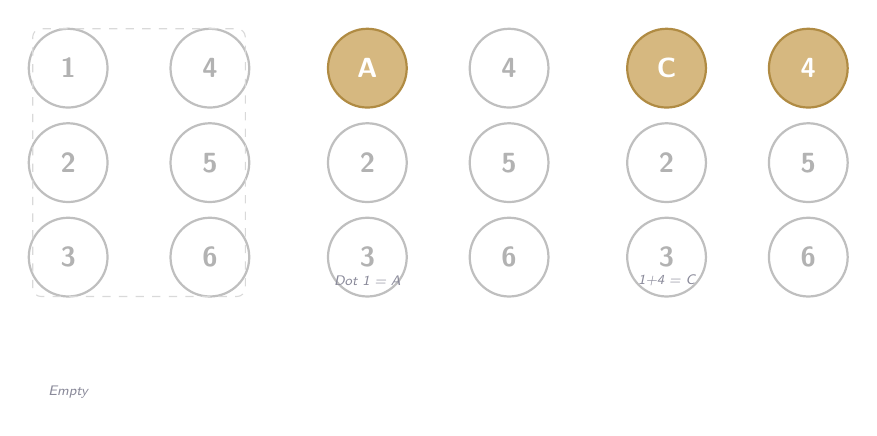
\begin{tikzpicture}[
  dot/.style={draw,circle,minimum size=10mm,inner sep=0pt,thick,font=\sffamily\bfseries},
  active/.style={fill=richgold!70,draw=richgold!90!black},
  inactive/.style={fill=white,draw=gray!50},
  label/.style={font=\tiny\sffamily\itshape,text=coolgrey}]

  \node[dot,inactive] (d1) at (0,2.4) {\color{gray!60}1};
  \node[dot,inactive] (d2) at (0,1.2) {\color{gray!60}2};
  \node[dot,inactive] (d3) at (0,0)   {\color{gray!60}3};
  \node[dot,inactive] (d4) at (1.8,2.4){\color{gray!60}4};
  \node[dot,inactive] (d5) at (1.8,1.2){\color{gray!60}5};
  \node[dot,inactive] (d6) at (1.8,0)  {\color{gray!60}6};
  \node[below=of d3,label] {Empty};

  \node[dot,active]  at (3.8,2.4) {\color{white}A};
  \node[dot,inactive]at (3.8,1.2) {\color{gray!60}2};
  \node[dot,inactive]at (3.8,0)   {\color{gray!60}3};
  \node[dot,inactive]at (5.6,2.4) {\color{gray!60}4};
  \node[dot,inactive]at (5.6,1.2) {\color{gray!60}5};
  \node[dot,inactive]at (5.6,0)   {\color{gray!60}6};
  \node[label] at (3.8,-0.3) {Dot 1 = A};

  \node[dot,active]  at (7.6,2.4) {\color{white}C};
  \node[dot,inactive]at (7.6,1.2) {\color{gray!60}2};
  \node[dot,inactive]at (7.6,0)   {\color{gray!60}3};
  \node[dot,active]  at (9.4,2.4) {\color{white}4};
  \node[dot,inactive]at (9.4,1.2) {\color{gray!60}5};
  \node[dot,inactive]at (9.4,0)   {\color{gray!60}6};
  \node[label] at (7.6,-0.3) {1+4 = C};

  \draw[rounded corners=3pt,gray!30,dashed] (-0.45,-0.5) rectangle (2.25,2.9);
\end{tikzpicture}
\caption{The six-dot Braille cell. Gold dots = active keys.}\label{fig:braille-cell}
\end{figure}

\subsection{First decade (A--J)}
Uses dots 1,2,4,5 only.\hfill
\begin{minipage}{0.45\textwidth}
\begin{tabular}{c c l}\toprule
\textbf{Letter} & \textbf{Chord} & \textbf{Dots} \\\midrule
A & 0b000001 & 1 \\
B & 0b000011 & 1,2 \\
C & 0b001001 & 1,4 \\
D & 0b011001 & 1,4,5 \\
E & 0b010001 & 1,5 \\\bottomrule
\end{tabular}
\end{minipage}\hfill
\begin{minipage}{0.45\textwidth}
\begin{tabular}{c c l}\toprule
\textbf{Letter} & \textbf{Chord} & \textbf{Dots} \\\midrule
F & 0b001011 & 1,2,4 \\
G & 0b011011 & 1,2,4,5 \\
H & 0b010011 & 1,2,5 \\
I & 0b001010 & 2,4 \\
J & 0b011010 & 2,4,5 \\\bottomrule
\end{tabular}
\end{minipage}

\subsection{Second decade (K--T)}
First-decade pattern + dot 3.\hfill
\begin{minipage}{0.45\textwidth}
\begin{tabular}{c c l}\toprule
\textbf{Letter} & \textbf{Chord} & \textbf{Base + 3} \\\midrule
K & 0b000101 & A+3 (1,3) \\
L & 0b000111 & B+3 (1,2,3) \\
M & 0b001101 & C+3 (1,3,4) \\
N & 0b011101 & D+3 (1,3,4,5) \\
O & 0b010101 & E+3 (1,3,5) \\\bottomrule
\end{tabular}
\end{minipage}\hfill
\begin{minipage}{0.45\textwidth}
\begin{tabular}{c c l}\toprule
\textbf{Letter} & \textbf{Chord} & \textbf{Base + 3} \\\midrule
P & 0b001111 & F+3 (1,2,3,4) \\
Q & 0b011111 & G+3 (1--5) \\
R & 0b010111 & H+3 (1,2,3,5) \\
S & 0b001110 & I+3 (2,3,4) \\
T & 0b011110 & J+3 (2,3,4,5) \\\bottomrule
\end{tabular}
\end{minipage}

\subsection{Third decade (U--Z)}
First-decade + dots 3 and 6. W is exception (2,4,5,6).

\begin{table}[H]\centering
\caption{Third decade U--Z.}\label{tab:english-third}
\begin{tabular}{c c l}\toprule
\textbf{Letter} & \textbf{Chord} & \textbf{Dots} \\\midrule
U & 0b100101 & 1,3,6 \\
V & 0b100111 & 1,2,3,6 \\
W & 0b111010 & 2,4,5,6 (exception) \\
X & 0b101101 & 1,3,4,6 \\
Y & 0b111101 & 1,3,4,5,6 \\
Z & 0b101001 & 1,3,5,6 \\\bottomrule
\end{tabular}\end{table}

%% 9 — BANGLA BRAILLE
\section{Bangla (Bharati) Braille Dictionary}

\projectname{} enters Bangla through Bharati Braille, the unified
South-Asian standard that maps Braille cells to \emph{sounds} rather than
to Latin letters. Because Bengali shares its phonetic basis with
international Braille, many cells coincide with their English counterparts
(e.g.\ \bengali{অ} = dot~1, like English~A), so the same six physical keys
serve both languages --- only the active dictionary changes. Bengali
numbers reuse the English number chords (Shift + A--J); the paper-Braille
numeric indicator is unnecessary because Shift already signals a digit.

\subsection{Vowels (\bengali{স্বরবর্ণ})}
Bharati Braille maps the ten Bengali vowels to dot patterns that follow
international phonetic conventions. For example, \bengali{অ} (short~o)
shares dot~1 with English~A, while \bengali{এ} (long~e) uses dots~1+5,
the same pattern as English~E. Vowels without an English parallel, such
as \bengali{আ} and \bengali{ঐ}, use dedicated Bharati cells. Dependent
vowel signs (\bengali{কার}) are produced by holding Shift while entering
the corresponding vowel chord in Bangla mode (Section~\ref{sec:bangla-kar}).

\begin{table}[H]\centering
\caption{Bangla vowel mappings (Bharati).}\label{tab:bangla-vowels}
\begin{minipage}{0.46\textwidth}
\begin{tabular}{l c c c}\toprule
\textbf{Vowel} & \textbf{English} & \textbf{Dots} & \textbf{Binary} \\midrule
অ (O)   & A     & 1       & 0b000001 \\
আ (Aa)  & ---   & 3,4,5   & 0b011100 \\
ই (I)   & I     & 2,4     & 0b001010 \\
ঈ (Long I) & --- & 3,5    & 0b010100 \\
উ (U)   & U     & 1,3,6   & 0b100101 \\bottomrule
\end{tabular}
\end{minipage}\hfill
\begin{minipage}{0.46\textwidth}
\begin{tabular}{l c c c}\toprule
\textbf{Vowel} & \textbf{English} & \textbf{Dots} & \textbf{Binary} \\midrule
ঊ (Long U) & --- & 1,2,5,6 & 0b110011 \\
এ (E)   & E     & 1,5     & 0b010001 \\
ঐ (Oi)  & ---   & 3,4     & 0b001100 \\
ও (O)   & O     & 1,3,5   & 0b010101 \\
ঔ (Ou)  & ---   & 2,4,6   & 0b101010 \\bottomrule
\end{tabular}
\end{minipage}
\end{table}

\subsection{Consonants (\bengali{ব্যঞ্জনবর্ণ})}
Bengali consonants are traditionally grouped into five \emph{varga} classes
(velar, palatal, retroflex, dental, labial) followed by a set of
semi-vowels and sibilants. Bharati Braille follows this phonetic order,
so the table below is grouped by varga exactly as the dictionary is
stored in firmware. Several cells match international Braille
(\bengali{ক} = dots~1,3 like K; \bengali{গ} = dots~1,2,4,5 like G).

\begin{table}[H]\centering
\caption{Bangla consonant mappings (Bharati), grouped by varga.}\label{tab:bangla-consonants}
\begin{minipage}{0.46\textwidth}
\begin{tabular}{l c c}\toprule
\textbf{ক-বর্গ (Velar)} & \textbf{Dots} & \textbf{Binary} \\midrule
ক (Ko) & 1,3   & 0b000101 \\
খ (Kho) & 4,6  & 0b101000 \\
গ (Go) & 1,2,4,5 & 0b011011 \\
ঘ (Gho) & 1,2,6 & 0b100011 \\
ঙ (Ngo) & 3,4,6 & 0b101100 \\bottomrule
\end{tabular}
\end{minipage}\hfill
\begin{minipage}{0.46\textwidth}
\begin{tabular}{l c c}\toprule
\textbf{চ-বর্গ (Palatal)} & \textbf{Dots} & \textbf{Binary} \\midrule
চ (Cho) & 1,4  & 0b001001 \\
ছ (Chho) & 1,6 & 0b100001 \\
জ (Jo) & 2,4,5 & 0b011010 \\
ঝ (Jho) & 3,5,6 & 0b110100 \\
ঞ (Nyo) & 2,5  & 0b010010 \\bottomrule
\end{tabular}
\end{minipage}

\vspace{0.6em}
\begin{minipage}{0.46\textwidth}
\begin{tabular}{l c c}\toprule
\textbf{ট-বর্গ (Retroflex)} & \textbf{Dots} & \textbf{Binary} \\midrule
ট (To) & 2,3,4,5,6 & 0b111110 \\
ঠ (Tho) & 2,4,5,6 & 0b110110 \\
ড (Do) & 1,2,4,6 & 0b101011 \\
ঢ (Dho) & All 6 & 0b111111 \\
ণ (No) & 3,4,5,6 & 0b111100 \\bottomrule
\end{tabular}
\end{minipage}\hfill
\begin{minipage}{0.46\textwidth}
\begin{tabular}{l c c}\toprule
\textbf{ত-বর্গ (Dental)} & \textbf{Dots} & \textbf{Binary} \\midrule
ত (To) & 2,3,4,5 & 0b011110 \\
থ (Tho) & 1,4,5,6 & 0b111001 \\
দ (Do) & 1,4,5 & 0b011001 \\
ধ (Dho) & 2,3,4,6 & 0b101110 \\
ন (No) & 1,3,4,5 & 0b011101 \\bottomrule
\end{tabular}
\end{minipage}

\vspace{0.6em}
\begin{minipage}{0.46\textwidth}
\begin{tabular}{l c c}\toprule
\textbf{প-বর্গ (Labial)} & \textbf{Dots} & \textbf{Binary} \\midrule
প (Po) & 1,2,3,4 & 0b001111 \\
ফ (Pho) & 2,3,5 & 0b010110 \\
ব (Bo) & 1,2   & 0b000011 \\
ভ (Bho) & 4,5  & 0b011000 \\
ম (Mo) & 1,3,4 & 0b001101 \\bottomrule
\end{tabular}
\end{minipage}\hfill
\begin{minipage}{0.46\textwidth}
\begin{tabular}{l c c}\toprule
\textbf{অন্যান্য (Semi-vowels)} & \textbf{Dots} & \textbf{Binary} \\midrule
য (Yo) & 1,3,4,5,6 & 0b111101 \\
র (Ro) & 1,2,3,5 & 0b010111 \\
ল (Lo) & 1,2,3 & 0b000111 \\
শ (Sha) & 1,4,6 & 0b101001 \\
ষ (Sha) & 1,2,3,4,6 & 0b101111 \\
স (Sa) & 2,3,4 & 0b001110 \\
হ (Ho) & 1,2,5 & 0b010011 \\bottomrule
\end{tabular}
\end{minipage}
\end{table}

\subsection{Shift + Vowel = Vowel Signs (\bengali{কার})}\label{sec:bangla-kar}
In Bangla mode, holding Shift while entering a vowel chord produces the
corresponding dependent vowel sign (\bengali{কার}) instead of the
independent vowel letter. Vowel signs always attach to a preceding
consonant, e.g.\ \bengali{ক} + \bengali{া} = \bengali{কা}. The chord is
identical to the parent vowel, so no extra memorisation is required.

\begin{table}[H]\centering
\caption{Bangla vowel signs (Shift + vowel).}\label{tab:bangla-vowelsigns}
\begin{minipage}{0.46\textwidth}
\begin{tabular}{l c c}\toprule
\textbf{Vowel} & \textbf{Vowel sign} & \textbf{Unicode} \\midrule
অ & া (Aa-kar)  & U+09BE \\
ই & ি (I-kar)   & U+09BF \\
ঈ & ী (Long I-kar) & U+09C0 \\
উ & ু (U-kar)   & U+09C1 \\
ঊ & ূ (Long U-kar) & U+09C2 \\bottomrule
\end{tabular}
\end{minipage}\hfill
\begin{minipage}{0.46\textwidth}
\begin{tabular}{l c c}\toprule
\textbf{Vowel} & \textbf{Vowel sign} & \textbf{Unicode} \\midrule
এ & ে (E-kar)   & U+09C7 \\
ঐ & ৈ (Oi-kar)  & U+09C8 \\
ও & ো (O-kar)   & U+09CB \\
ঔ & ৌ (Ou-kar)  & U+09CC \\bottomrule
\end{tabular}
\end{minipage}
\end{table}

\subsection{Special Marks}
Four auxiliary marks complete the Bangla set. The halant (\bengali{্})
suppresses the inherent vowel and forms conjuncts, the anusvara
(\bengali{ং}) nasalises, the visarga (\bengali{ঃ}) adds aspiration, and
the candrabindu (\bengali{ঁ}) marks nasalised vowels. Each is entered
with its own chord.

\begin{table}[H]\centering
\caption{Bangla special marks.}\label{tab:bangla-marks}
\begin{tabular}{l c c c}\toprule
\textbf{Mark} & \textbf{Name} & \textbf{Dots} & \textbf{Binary} \\midrule
্ & Halant (virama)   & 4     & 0b001000 \\
ং & Anusvara          & 5,6   & 0b110000 \\
ঃ & Visarga           & 6     & 0b100000 \\
ঁ & Candrabindu       & 5     & 0b010000 \\bottomrule
\end{tabular}\end{table}

\section{Numbers, Punctuation and Mathematics}

Shift provides access to numbers, punctuation, and math symbols.

\subsection{Numbers}
Numbers reuse the first-decade letter chords (A--J) with Shift held, in the
same tradition as the paper-Braille numeric indicator: the chord for~A
with Shift gives~1, B gives~2, and so on up to J giving~0. Because Shift
already signals a digit, no separate numeric-indicator cell is needed ---
the modifier does the job.

\begin{table}[H]\centering
\caption{Number mappings.}\label{tab:numbers}
\begin{tabular}{c c c}\toprule
\textbf{Shift +} & \textbf{Number} & \textbf{Dots} \\\midrule
A & 1 & 1 \\
B & 2 & 1,2 \\
C & 3 & 1,4 \\
D & 4 & 1,4,5 \\
E & 5 & 1,5 \\
F & 6 & 1,2,4 \\
G & 7 & 1,2,4,5 \\
H & 8 & 1,2,5 \\
I & 9 & 2,4 \\
J & 0 & 2,4,5 \\\bottomrule
\end{tabular}\end{table}

\subsection{Punctuation}
Punctuation is entered with Shift held while pressing the chord, exactly
like numbers. The punctuation set covers everyday writing needs; the
period chord (2,5,6) doubles as the decimal point in mathematical work.

\begin{table}[H]\centering
\caption{Punctuation mappings.}\label{tab:punctuation}
\begin{tabular}{c c c}\toprule
\textbf{Symbol} & \textbf{Name} & \textbf{Dots} \\\midrule
, & Comma & 2 \\
; & Semicolon & 2,3 \\
: & Colon & 2,5 \\
. & Period / decimal point & 2,5,6 \\\bottomrule
\end{tabular}\end{table}

Question mark (dots 2,3,6) and exclamation point (dots 2,3,5) chords
are reserved in the same Shift layer and can be added without any
hardware change --- the dictionary is data, not control flow.

\subsection{Mathematical Symbols}
The most commonly needed operators are mapped onto Shift chords using
the standard Bharati/UEB cell values, so a student can type a full
arithmetic expression without leaving the keyboard:

\begin{table}[H]\centering
\caption{Mathematical symbol mappings.}\label{tab:math-symbols}
\begin{tabular}{c c c}\toprule
\textbf{Symbol} & \textbf{Name} & \textbf{Dots} \\\midrule
$+$ & Plus (\bengali{যোগ}) & 2,3,5 \\
$-$ & Minus (\bengali{বিয়োগ}) & 3,6 \\
$\times$ & Multiplication (\bengali{গুণ}) & 2,3,6 \\
$\div$ & Division (\bengali{ভাগ}) & 3,4 \\
$=$ & Equals (\bengali{সমান}) & 2,3,5,6 \\\bottomrule
\end{tabular}\end{table}

Because the operators live in the Shift layer, a student can alternate
between digits (Shift + A--J) and operators without ever leaving a
mathematical context --- a significant advantage over dictating
arithmetic to a sighted writer.

%% 11 — TEACHER SOFTWARE
\section{Teacher Software --- Web Application}

Built with HTML, CSS, and JavaScript using the Web Serial API. Runs in
Chrome / Edge. No Python, no Qt, no SQLite --- a browser is sufficient.

\subsection{Architecture}
The application is a single-page web app: no backend, no database, and
no installation --- the browser talks directly to each ESP32 over the
Web Serial API. Data flows through one pipeline:

\begin{quote}\small
Web Serial API $\rightarrow$ serial reader loop (115200 baud) $\rightarrow$
protocol parser (LANG:en/bn, chars) $\rightarrow$ student data store
(chars + timestamps) $\rightarrow$ DOM renderers (feed, exam, expand
views) $\rightarrow$ export engine (TXT with timestamps).
\end{quote}

Because everything runs client-side, a teacher's computer is the only
infrastructure required. The same HTML file works for one student or a
full classroom --- students are added as data rows, not as code changes.

\subsection{Key Features}
\begin{itemize}[nosep]
  \item Multi-student roster: add students, assign COM ports, set baud rates.
  \item Live serial reading with dedicated reader loop per student.
  \item Language detection from \texttt{LANG:en}/\texttt{LANG:bn} messages.
  \item Real-time serif-font display with auto-scroll and blinking cursor.
  \item Teacher feed cards: avatar, name, connection status, language, stats.
  \item Expand modal: full-screen 64px serif text overlay for close monitoring.
  \item Exam mode: grid layout with all students side-by-side.
  \item Chord visualization: 6 mini-dots animate per chord input.
  \item Timestamped export: \texttt{[HH:MM:SS]} prefix per character.
  \item Light/dark theme with \texttt{Ctrl+Shift+T} shortcut.
  \item Persistent roster via \texttt{localStorage}.
\end{itemize}

\subsection{Serial Connection (Web Serial API)}
\begin{lstlisting}[language=JavaScript,caption=Connecting to a BrailleBridge device.]
async function connectStudentSerial(student) {
  const port = await navigator.serial.requestPort();
  await port.open({ baudRate: student.baud });
  student.serialPort = port; student.connected = true;

  const decoder = new TextDecoderStream();
  port.readable.pipeTo(decoder.writable);
  const reader = decoder.readable.getReader();

  async function readLoop() {
    while (student.readLoopActive) {
      const { value, done } = await reader.read();
      if (done) break;
      for (const ch of value) handleStudentChar(student, ch);
    }
  }
  readLoop();
}
\end{lstlisting}

\subsection{Character Pipeline}
Every character that arrives from a student's ESP32 passes through a
single \texttt{handleStudentChar} pipeline. The routine validates the
byte, attaches a millisecond-precision timestamp, appends it to the
student's stored history, and then updates every rendered view --- the
teacher feed card, the exam grid, and the expand modal --- in one pass.

A 500\,ms interval timer rebuilds all feeds directly from the stored
history as a failsafe, so even if a DOM update is missed or the browser
re-renders, no character is ever lost from the record. This design keeps
the live view simple while the persistent store remains the single
source of truth.

\subsection{Timestamped Export}
Each stored character is a \texttt{\{char, time\}} pair with
millisecond precision. Exporting a student's work produces a plain-text
\texttt{.txt} file (named \texttt{braillebridge-\{student\}.txt}) in which
every character is prefixed with its wall-clock time:

\begin{verbatim}
[09:12:01] T
[09:12:01] h
[09:12:02] e
[09:12:03]   
[09:12:04] a
[09:12:05] n
\end{verbatim}

The timestamp column lets a teacher see not just what a student wrote,
but the pace and order of composition --- useful for assessing
fluency, spotting hesitation, or reconstructing how an examination
answer was built up.

\subsection{Visual Design}
The Teacher Software is designed as professional educational software
rather than a hobbyist dashboard. Typography uses serif faces (Georgia
for Latin, Noto Serif Bengali for Bangla) chosen for legibility at
exam-appropriate sizes. The default theme is a warm dark palette with a
gold accent (\#C49A4A) and colour-coded student avatars; a full light
mode is one click (or \texttt{Ctrl+Shift+T}) away, and the choice is
remembered between sessions.

Deliberately, no emojis appear anywhere --- all status, connection, and
action indicators use Font Awesome icons, keeping the interface calm and
professional for exam invigilation. The expand modal renders a student's
feed in 64px serif text for close reading, and the exam view arranges
all students side-by-side in a grid so a single teacher can monitor an
entire class at a glance.

%% 12 — ENGINEERING INNOVATIONS
\section{Engineering Innovations}

\begin{itemize}[nosep]
  \item \textbf{Chord buffering:} 180\,ms window solves the problem of
    fingers landing milliseconds apart.
  \item \textbf{Bitmask encoding:} Six keys represented as one 6-bit integer
    for compact, constant-time comparison.
  \item \textbf{Dictionary-based translation:} Adding a new language requires
    only array entries --- no control-flow changes.
  \item \textbf{Dual communication:} Bluetooth for student, USB Serial for
    teacher --- simultaneous, independent channels.
  \item \textbf{Software-defined language:} No hardware switch needed ---
    a boolean variable selects English or Bangla.
  \item \textbf{Modifier architecture:} Shift expands output range (caps,
    numbers, symbols) without adding physical keys.
  \item \textbf{Modular construction:} Switches, ESP32, enclosure, and
    software are independently repairable/upgradable.
  \item \textbf{Web-based Teacher Software:} No install required --- runs
    in the browser, updates on refresh.
  \item \textbf{Failsafe refresh:} 500\,ms interval rebuilds all feeds
    from stored data, ensuring no character is lost.
\end{itemize}

%% 13 — COMPARATIVE ANALYSIS
\section{Comparative Analysis}

\begin{longtable}{p{2.5cm} p{3.5cm} p{5.5cm}}
\caption{Comprehensive comparison with existing solutions.}\label{tab:comprehensive}\\\toprule
\textbf{Solution} & \textbf{Strengths} & \textbf{Weaknesses} \\\midrule
\endfirsthead
\toprule\textbf{Solution} & \textbf{Strengths} & \textbf{Weaknesses}\\\midrule
\endhead
\bottomrule\endfoot
Human writer & No equipment & Privacy loss, errors \\
Slate \& stylus & Affordable, tactile & Unreadable to sighted teachers \\
Perkins Brailler & Familiar method & \$600--\$1000+, heavy, embossed only \\
Voice typing & Fast in quiet & Fails in noise, poor for math \\
Commercial digital & Advanced accessibility & \$1000--\$5000+, hard to repair \\
Ordinary keyboard & Cheap & No six-dot chording \\
\rowcolor{lineshade}\projectname{} & Bilingual + teacher software & Prototype stage \\
\end{longtable}

%% 14 — AFFORDABILITY
\section{Affordability}

\begin{table}[H]\centering
\caption{Approximate bill of materials per device.}\label{tab:bom}
\begin{tabular}{l r r}\toprule
\textbf{Component} & \textbf{Qty} & \textbf{Cost (USD)} \\\midrule
ESP32 Dev Module & 1 & \$5.00 \\
Outemu Red switch & 8 & \$3.00 \\
Keycaps (3D-printed) & 8 & \$1.00 \\
LED (3mm) + resistor & 2+2 & \$0.30 \\
Perfboard & 1 & \$0.80 \\
PLA filament (enclosure) & 30g & \$1.20 \\
M3 screws, wire, solder & -- & \$0.70 \\
\midrule\textbf{Total} & & \textbf{\textasciitilde{}\$12.00} \\\bottomrule
\end{tabular}\end{table}

Even including tools and overhead, a complete device costs under \$15 --- a
fraction of mechanical Braillers or commercial digital systems. Schools can
deploy multiple units, and damaged components (switches, ESP32) are replaced
for a few dollars each.

%% 15 — CONCLUSION
\section{Conclusion}

\projectname{} addresses a specific educational problem: blind students
cannot independently produce written answers that their sighted teachers
can read. The project combines a physical Braille chord keyboard, an
ESP32-based translator, and a web-based teacher application into a
complete, affordable classroom system.

\projectname{} is innovative because it integrates proven technologies ---
six-dot chording, an ESP32, Bluetooth HID, the Web Serial API --- into a
solution that bridges four gaps:

\begin{enumerate}[nosep]
  \item Between the blind student's tactile writing and the teacher's
    need for readable text.
  \item Between English and Bangla Braille.
  \item Between the student's independent composition and the teacher's
    assessment workflow.
  \item Between the high cost of commercial assistive technology and
    limited school budgets.
\end{enumerate}

The most important measure is practical impact: when a blind student writes
her own examination answer for the first time, without a writer, without
speaking aloud, and without the teacher needing Braille, the project has
succeeded.

\vspace{1cm}\begin{center}
\itshape\large``BrailleBridge does not replace Braille.\\
It protects Braille as the student's natural writing method\\
while removing the barrier between Braille input\\
and teacher-readable output.''
\end{center}

\vspace{0.5cm}\noindent\textbf{References:} \\
[1] \href{https://www.espressif.com/en/products/socs/esp32}{Espressif Systems --- ESP32 Series Datasheet} --- \url{https://www.espressif.com/en/products/socs/esp32}. \\
[2] \href{https://en.wikipedia.org/wiki/Bharati_Braille}{Bharati Braille --- Wikipedia} --- \url{https://en.wikipedia.org/wiki/Bharati_Braille}. \\
[3] \href{https://en.wikipedia.org/wiki/English_Braille}{English Braille --- Wikipedia} --- \url{https://en.wikipedia.org/wiki/English_Braille}. \\
[4] \href{https://developer.mozilla.org/en-US/docs/Web/API/Web_Serial_API}{MDN Web Docs --- Web Serial API} --- \url{https://developer.mozilla.org/en-US/docs/Web/API/Web_Serial_API}. \\
[5] \href{https://github.com/espressif/arduino-esp32}{Arduino core for ESP32 --- GitHub} --- \url{https://github.com/espressif/arduino-esp32}. \\
[6] \href{https://github.com/T-vK/ESP32-BLE-Keyboard}{ESP32 Bluetooth Keyboard Library --- GitHub} --- \url{https://github.com/T-vK/ESP32-BLE-Keyboard}. \\
[7] World Braille Usage, UNESCO / NLS, 3rd ed., 2013.

\end{document}
